% Final report – LaTeX version of docs/final_report.md
% Build:  latexmk -pdf report.tex   (run inside docs/latex/)
\documentclass[11pt,a4paper]{article}

\usepackage[T1,T5]{fontenc}
\usepackage[utf8]{inputenc}
\usepackage{lmodern}
\usepackage[vietnamese,main=english]{babel}
\usepackage{microtype}
\usepackage[margin=2.5cm]{geometry}
\usepackage{amsmath,amssymb}
\usepackage{graphicx}
\usepackage{booktabs}
\usepackage{tabularx}
\usepackage{array}
\usepackage{float}
\usepackage{caption}
\usepackage{subcaption}
\usepackage{xcolor}
\usepackage{listings}
\usepackage{tikz}
\usetikzlibrary{arrows.meta,positioning,calc}
\usepackage{siunitx}
\usepackage{enumitem}
\usepackage[hidelinks]{hyperref}

\graphicspath{{../figures/}{figures/}}
\sisetup{group-separator={\,},group-minimum-digits=4}
\setlength{\emergencystretch}{3em}

\definecolor{codebg}{HTML}{F6F6F4}
\definecolor{accent}{HTML}{1F5FA8}
\definecolor{warn}{HTML}{D2691E}
\lstset{
  basicstyle=\ttfamily\footnotesize,
  backgroundcolor=\color{codebg},
  keywordstyle=\color{accent}\bfseries,
  commentstyle=\color{gray}\itshape,
  frame=single, rulecolor=\color{gray!40},
  columns=fullflexible, keepspaces=true,
  breaklines=true, xleftmargin=4pt, xrightmargin=4pt,
  aboveskip=8pt, belowskip=8pt
}
\lstdefinestyle{cpp}{language=C++,morekeywords={pragma,omp,parallel,for,schedule,runtime,nowait}}

\newcommand{\x}{\ensuremath{\times}}
\newcommand{\us}{\,\textmu s}
\newcommand{\calc}{\emph{(calculation)}}

\title{\textbf{Parallel Implementation of Seam Carving for\\Content-Aware Image Resizing using OpenMP}\\[6pt]
\large Final Project Report -- Parallel Computing}
\author{Đỗ Tùng Dương \quad Hoàng Trọng Đại \quad Lê Quang Huy\\[2pt]
\small MAT3148 -- Tính Toán Song Song (Parallel Computing)\\
\small VNU University of Science (VNU-HUS)}
\date{26/11/2026}

\begin{document}
\maketitle

\begin{center}
\small Repository: \texttt{MyleCutie45/TTSS} \quad Language: C++17 \quad Parallel framework: OpenMP \quad Build: CMake
\end{center}

\begin{abstract}
Seam carving (Avidan and Shamir, 2007) shrinks an image by repeatedly removing a connected path of
low-energy pixels, so that salient content keeps its shape. Each removal requires an energy map, a
dynamic-programming (DP) pass over the whole image, a backtracking step and a pixel shift, and the
removals form a strictly sequential chain. This report describes three implementations that produce
bit-identical results: a sequential baseline, a direct OpenMP parallelization of each stage, and an
optimized OpenMP version. On an Intel Core i7-1065G7 under Windows, the direct parallelization is slower
than the sequential program whenever the DP is parallel, because every image row requires a barrier that
costs 22--167\us{} in the Windows build of the OpenMP runtime; with the DP kept sequential it reaches
1.40--1.79\x. The optimized version removes redundant work (incremental energy update, vectorizable
kernels), reduces memory traffic (16-bit energy, 1-byte backtracking directions) and replaces the per-row
barrier by one barrier per block of 64 rows with redundant ``halo'' computation. On an AMD Ryzen 7 4800H
(Linux container) it is 4.4--4.8\x{} faster than the sequential program with 8 threads, compared with
1.5--1.6\x{} for the direct parallelization on the same machine. The remaining limit is the memory
bandwidth of the seam-removal stage.
\end{abstract}

\tableofcontents
\newpage

% ---------------------------------------------------------------------------
\section{Introduction}

Content-aware image resizing changes the aspect ratio of an image without uniformly scaling or cropping
it. Seam carving achieves this by deleting, one at a time, the 8-connected path of pixels (``seam'') whose
summed gradient energy is minimal (Figure~\ref{fig:compare}). The method is simple, but expensive: removing
$k$ seams from a $W\times H$ image costs $\Theta(k\,W\,H)$ operations, and the $k$ removals cannot be
performed independently, because each seam depends on the image left by the previous one.

\begin{figure}[ht]
  \centering
  \begin{subfigure}[b]{0.36\textwidth}\centering
    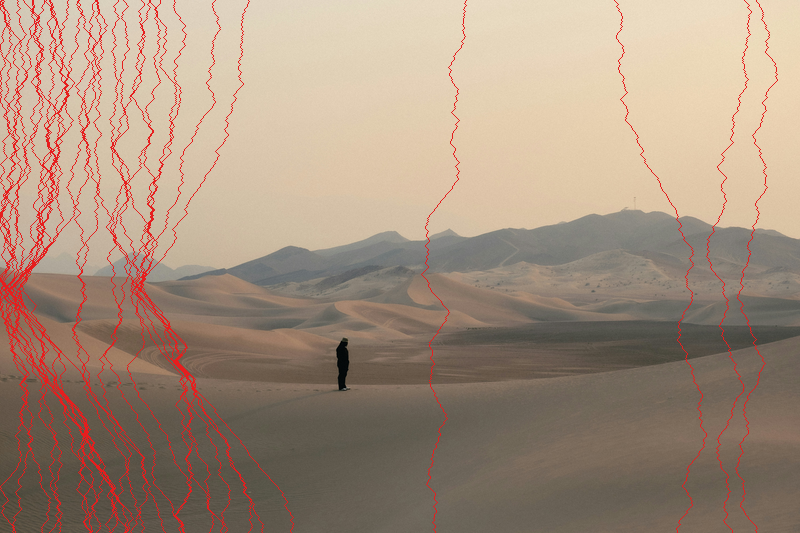
\includegraphics[width=\linewidth]{seams.png}\caption{Input $800\times533$, first 30 seams}\end{subfigure}\hfill
  \begin{subfigure}[b]{0.20\textwidth}\centering
    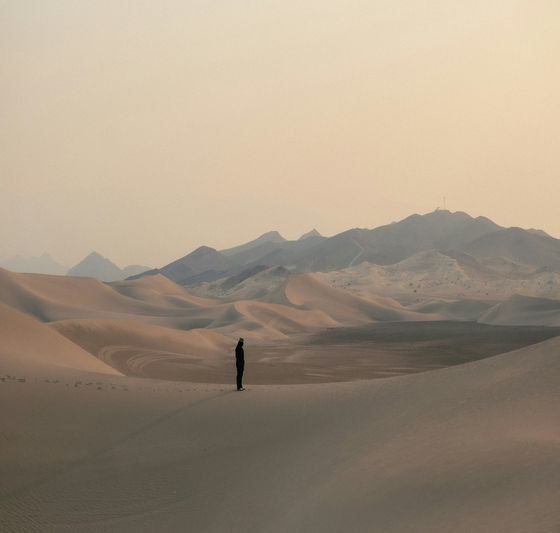
\includegraphics[width=\linewidth]{scaled.png}\caption{Scaled}\end{subfigure}\hfill
  \begin{subfigure}[b]{0.20\textwidth}\centering
    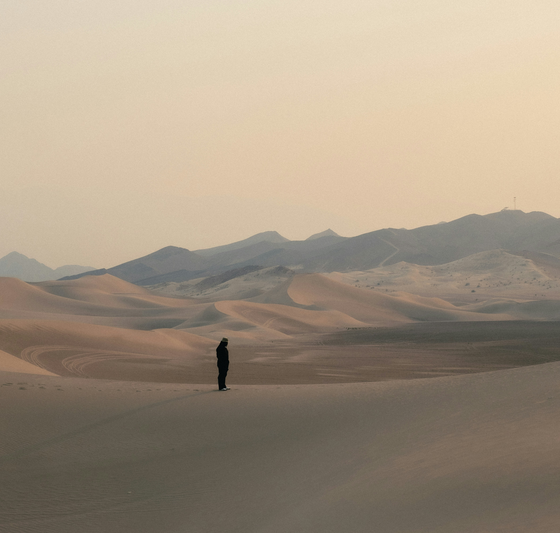
\includegraphics[width=\linewidth]{cropped.png}\caption{Cropped}\end{subfigure}\hfill
  \begin{subfigure}[b]{0.20\textwidth}\centering
    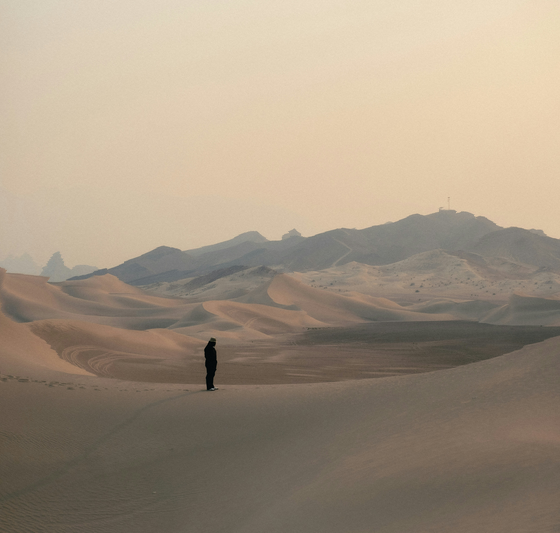
\includegraphics[width=\linewidth]{carved.png}\caption{Seam carved}\end{subfigure}
  \caption{Reducing the width from 800 to 560 pixels. (d) is the output of our program
  (\texttt{--mode opt}); the red seams in (a) were drawn with an illustrative NumPy re-implementation
  of the same rules (\texttt{scripts/make\_latex\_figures.py}). Photo: Unsplash, see
  \texttt{images/SOURCES.md}.}
  \label{fig:compare}
\end{figure}

The goal of this project is to study how far this algorithm can be accelerated on a shared-memory
multicore processor with OpenMP, and \emph{why} it does or does not scale. The project was organised in
seven milestones: research (M0), sequential implementation (M1), OpenMP implementation (M2),
correctness testing (M3), benchmarking (M4), optimization (M5) and this report (M6).

Contributions of the project:
\begin{enumerate}
  \item A sequential reference implementation with explicitly specified integer arithmetic and
        tie-breaking rules, so that every parallel variant can be compared bit for bit (Section~\ref{sec:seq}).
  \item A stage-by-stage OpenMP parallelization with switchable stages and two DP variants
        (Section~\ref{sec:omp}).
  \item A measurement-based explanation of why the parallel DP fails on Windows (synchronization cost) and
        why it scales poorly even where synchronization is cheap (memory traffic)
        (Sections~\ref{sec:perf}--\ref{sec:bottle}).
  \item An optimized version whose every optimization can be switched off and was measured in isolation
        (Section~\ref{sec:opt}).
\end{enumerate}

\paragraph{Original research vs.\ our work.} The seam definition, the energy function $e_1$, the DP
recurrence and the use of transposition for horizontal seams come from Avidan and Shamir (2007). Every
implementation decision (integer energy without normalisation, clamped borders, tie rules, the
parallelization, all optimizations) and every measurement in this report is our own work;
Table~\ref{tab:origin} lists them.

\begin{table}[ht]
\centering\small
\begin{tabularx}{\textwidth}{@{}l>{\raggedright\arraybackslash}p{4.2cm}>{\raggedright\arraybackslash}X@{}}
\toprule
Topic & From the original paper & Our decision \\
\midrule
Energy & $e_1=|\partial I/\partial x|+|\partial I/\partial y|$ & central differences without division by 2,
  on the gray image, clamped at borders, 32-bit integers (16-bit in M5) \\
Seam & 8-connected, one pixel per row & same \\
Optimal seam & DP over cumulative energy $M$ & same recurrence; ties: smallest column wins (endpoint and backtracking) \\
Repeated removal & recompute after each seam & M1/M2: full recomputation; M5: provably equivalent local update \\
Height reduction & transpose & transpose after the width has been reduced \\
Seam order, enlarging, masks, multi-size images & described in the paper & out of scope \\
Parallelization, synchronization, optimization & not addressed & Sections~\ref{sec:strategy}--\ref{sec:opt} \\
\bottomrule
\end{tabularx}
\caption{What comes from the original paper and what was decided in this project.}
\label{tab:origin}
\end{table}

% ---------------------------------------------------------------------------
\section{Problem Statement}

Given a color image $I$ of size $W\times H$ and a target size $W'\times H'$ with $W'\le W$, $H'\le H$,
produce the image obtained by removing $W-W'$ vertical seams and then $H-H'$ horizontal seams, each time
the seam of minimal energy, \textbf{exactly as the sequential algorithm does}. The parallel program must:
\begin{itemize}
  \item produce an output that is bit-identical to the sequential output for every image, target size,
        thread count and schedule (determinism);
  \item be faster than the sequential program on a multicore CPU, and the speedup must be explained by
        measurements;
  \item keep the sequential program as an unchanged correctness baseline.
\end{itemize}

The difficulty is structural. Of the five stages executed for every seam (Section~\ref{sec:algo}), two are
embarrassingly parallel (energy, removal), one is a reduction (minimum), one is an inherently sequential
chain (backtracking), and the most expensive one, the DP, has a row-to-row dependency that allows
parallelism only \emph{within} a row. Moreover, all stages are executed thousands of times on the same
data with little arithmetic per pixel, so synchronization and memory traffic, not computation, decide the
performance.

% ---------------------------------------------------------------------------
\section{Background and Related Work}

\paragraph{Seam carving.} Avidan and Shamir~\cite{avidan2007} introduced seams as monotone, 8-connected
paths and showed that the optimal seam under an additive energy can be found by dynamic programming in
$O(W\cdot H)$. They compared several energy functions (gradient magnitude $e_1$, entropy, histogram of
gradients) and proposed an optimal ordering of vertical and horizontal removals, seam insertion for
enlarging, and object removal. Rubinstein, Shamir and Avidan~\cite{rubinstein2008} introduced
\emph{forward energy}, which measures the energy inserted by a removal, and graph-cut formulations for
video. This project implements the basic backward-energy ($e_1$) algorithm, which is the common baseline.

\paragraph{OpenMP.} OpenMP~\cite{openmp52} is a directive-based shared-memory programming model. A
\texttt{parallel} region creates a team of threads; work-sharing constructs (\texttt{for}) divide loop
iterations among them according to a \emph{schedule} (\texttt{static}, \texttt{dynamic},
\texttt{guided}); an implicit \emph{barrier} at the end of a work-sharing loop ensures that all iterations
are finished before any thread continues. The \texttt{simd} construct asks the compiler to vectorize a
loop, and the \texttt{if} clause executes a region serially when a condition is false~\cite{chapman2008}.

\paragraph{Performance models.} Amdahl's law~\cite{amdahl1967} bounds the speedup of a program with a
serial fraction $f$ by $1/(f+(1-f)/p)$. For memory-intensive kernels, the attainable performance is
bounded by the product of arithmetic intensity and memory bandwidth (the \emph{roofline}
model~\cite{williams2009}); we measure the bandwidth with a STREAM-like kernel~\cite{mccalpin1995}.

\paragraph{Wavefront and overlapped tiling.} The DP is a stencil-like recurrence in which row $y$ depends
on three cells of row $y-1$. The standard way to reduce synchronization in such iterative stencils is to
let each thread compute a slightly larger region than it owns (``ghost zones'' or overlapped tiles),
trading redundant computation for fewer barriers~\cite{meng2009}. Our blocked DP
(Section~\ref{sec:o3}) applies this idea to the seam-carving DP.

% ---------------------------------------------------------------------------
\section{Original Seam Carving Algorithm}
\label{sec:algo}

Let $I$ be the gray image and $W$ its current width.

\paragraph{Energy} (Avidan and Shamir's $e_1$):
\[
  e(x,y) = \left|\frac{\partial I}{\partial x}\right| + \left|\frac{\partial I}{\partial y}\right| .
\]

\paragraph{Vertical seam.} A seam is a set $s=\{(s(y),y) : y=0,\dots,H-1\}$ with $|s(y)-s(y-1)|\le 1$;
its cost is $E(s)=\sum_y e(s(y),y)$, and the optimal seam is $s^*=\arg\min_s E(s)$.

\paragraph{Dynamic programming.} The minimal cost of a seam ending at $(x,y)$ is
\[
  M(x,0)=e(x,0),\qquad
  M(x,y)=e(x,y)+\min\bigl(M(x-1,y-1),\;M(x,y-1),\;M(x+1,y-1)\bigr),
\]
where neighbours outside the image are ignored. The minimum of the last row is the cost of $s^*$, and the
seam is recovered by backtracking from that cell to row 0, always moving to the smallest upper neighbour.

\paragraph{Removal and repetition.} The seam pixel is deleted in each row and the pixels to its right are
shifted left, giving a $(W-1)\times H$ image. Energy and $M$ are recomputed for the next seam. Horizontal
seams are handled by transposing the image.

\paragraph{Worked example.} Table~\ref{tab:example} shows the $4\times4$ example used as a unit test
(\texttt{docs/algorithm.md}, \S5). The last row of $M$ has its minimum 140 at $x=0$; backtracking gives the
seam $s=[1,2,1,0]$ (row 0 has a tie between $x=1$ and $x=3$; the smallest column wins).

\begin{table}[ht]
\centering\small
\begin{tabular}{@{}c@{\hspace{2.5em}}c@{\hspace{2.5em}}c@{}}
Gray image $I$ & Energy $e$ & Cumulative energy $M$ \\[2pt]
\begin{tabular}{rrrr}\toprule 10&\textbf{20}&30&40\\ 50&10&\textbf{60}&20\\ 30&\textbf{70}&10&50\\ \textbf{20}&40&60&10\\\bottomrule\end{tabular} &
\begin{tabular}{rrrr}\toprule 50&\textbf{30}&50&30\\ 60&60&\textbf{30}&50\\ 70&\textbf{50}&20&50\\ \textbf{30}&70&80&90\\\bottomrule\end{tabular} &
\begin{tabular}{rrrr}\toprule 50&\textbf{30}&50&30\\ 90&90&\textbf{60}&80\\ 160&\textbf{110}&80&110\\ \textbf{140}&150&160&170\\\bottomrule\end{tabular}
\end{tabular}
\caption{Worked $4\times4$ example; the optimal seam (bold) has cost $30+30+50+30=140=M(0,3)$.}
\label{tab:example}
\end{table}

\paragraph{Complexity.} One seam costs $\Theta(W\cdot H)$; removing $k$ seams costs
\[
  \sum_{i=0}^{k-1}(W-i)\,H = k\,H\Bigl(W-\tfrac{k-1}{2}\Bigr)=\Theta(k\,W\,H).
\]

% ---------------------------------------------------------------------------
\section{Sequential Implementation}
\label{sec:seq}

The sequential program (\texttt{src/seam\_seq.cpp}, namespace \texttt{seq}, compiled \textbf{without}
OpenMP) executes five stages for every seam:

\begin{lstlisting}
function CARVE(image, targetWidth, targetHeight):
    gray  <- toGray(image)                          // once (OpenCV cvtColor)
    width <- image.cols
    while width > targetWidth:                      // k iterations, strictly sequential
        e   <- COMPUTE_ENERGY(gray, width)          // stage 1   Theta(W*H)
        M   <- COMPUTE_CUMULATIVE(e, width)         // stage 2   Theta(W*H), rows dependent
        end <- FIND_MIN_ENDPOINT(M[H-1], width)     // stage 3   Theta(W)
        s   <- BACKTRACK(M, end)                    // stage 4   Theta(H), dependent chain
        REMOVE_SEAM(image, gray, s, width)          // stage 5   Theta(W*H) memory moves
        width <- width - 1
    if targetHeight < H: transpose, repeat for rows, transpose back
    return image[:, 0 .. targetWidth-1]
\end{lstlisting}

Implementation decisions (all documented in \texttt{docs/algorithm.md}, decisions D1--D7):
\begin{itemize}
  \item \textbf{Integer arithmetic.} $e(x,y)=|I(x+1,y)-I(x-1,y)|+|I(x,y+1)-I(x,y-1)|$ with indices clamped
    to the image, without division by 2; the maximum is 510. $M$ fits easily into 32-bit integers
    ($510\cdot4320\approx2.2\cdot10^6$). Integer arithmetic makes the results independent of the
    evaluation order, which is the precondition for exact comparison of parallel results.
  \item \textbf{Deterministic ties.} The smallest column wins at the endpoint and in backtracking
    (candidates in the order $x-1, x, x+1$, strict \texttt{<}).
  \item \textbf{Current width.} All stages operate on columns $[0,\mathit{width})$ of matrices allocated
    once at the original size; the result is cropped at the end. No reallocation happens inside the seam
    loop.
  \item \textbf{Gray image updated, not recomputed.} The gray image is shifted together with the color
    image.
\end{itemize}

% ---------------------------------------------------------------------------
\section{Parallelization Strategy}
\label{sec:strategy}

The outer seam loop cannot be parallelized: seam $i+1$ is defined on the image produced by seam $i$. All
parallelism is therefore \emph{inside} one seam iteration (Figure~\ref{fig:pipeline}).

\begin{figure}[ht]
\centering
\begin{tikzpicture}[
  st/.style={draw, rounded corners=3pt, align=center, text width=2.2cm, minimum height=1.4cm, inner sep=3pt,
             font=\footnotesize, fill=#1},
  st/.default=accent!10,
  >=Stealth, node distance=0.32cm]
  \node[st] (E) {\textbf{1 Energy}\\rows independent\\\texttt{parallel for}};
  \node[st=warn!15, right=of E] (D) {\textbf{2 DP}\\row $y$ needs $y-1$\\parallel in a row};
  \node[st, right=of D] (M) {\textbf{3 Minimum}\\reduction};
  \node[st=gray!15, right=of M] (B) {\textbf{4 Backtrack}\\dependent chain\\sequential};
  \node[st, right=of B] (R) {\textbf{5 Removal}\\rows independent\\\texttt{parallel for}};
  \draw[->] (E) -- (D); \draw[->] (D) -- (M); \draw[->] (M) -- (B); \draw[->] (B) -- (R);
  \draw[->] (R.south) -- ++(0,-0.5) -| node[pos=0.25, below, font=\small]{next seam (repeated $k$ times, sequential)} (E.south);
\end{tikzpicture}
\caption{Stages of one seam and the parallelism available in each.}
\label{fig:pipeline}
\end{figure}

\begin{table}[ht]
\centering\small
\begin{tabularx}{\textwidth}{@{}l>{\raggedright\arraybackslash}X>{\raggedright\arraybackslash}X>{\raggedright\arraybackslash}X@{}}
\toprule
Stage & Dependency & Strategy (M2) & Synchronization per seam \\
\midrule
Energy & none between pixels & \texttt{parallel for} over rows & 1 region + 1 barrier \\
DP & row $y$ needs row $y-1$ & \texttt{for} over columns of each row & \textbf{1 barrier per row} ($H$ per seam) \\
Minimum & reduction over the last row & per-thread minimum, sequential combine & 1 region \\
Backtrack & $s(y-1)$ depends on $s(y)$ & sequential & -- \\
Removal & rows independent & \texttt{parallel for} over rows & 1 region + 1 barrier \\
\bottomrule
\end{tabularx}
\caption{Parallelization strategy of the direct OpenMP version (M2).}
\end{table}

The DP is the critical stage: for a $1920\times1080$ image and 384 seams it requires \num{414336}
synchronizations ($(1080-1)$ rows $\times$ 384 seams), each protecting only about 2\us{} of work
(Section~\ref{sec:why}).

% ---------------------------------------------------------------------------
\section{OpenMP Implementation}
\label{sec:omp}

The OpenMP version (\texttt{src/seam\_omp.cpp}, namespace \texttt{omp\_impl}) mirrors the sequential code
stage by stage; a \texttt{ParallelConfig} selects which stages run in parallel
(\texttt{--stages energy,dp,min,removal}) and which DP variant is used. All loops use
\texttt{schedule(runtime)}; the program sets \texttt{static} unless \texttt{OMP\_SCHEDULE} is defined.

\paragraph{Energy and removal} -- rows are independent; every iteration writes only row $y$:
\begin{lstlisting}[style=cpp]
#pragma omp parallel for schedule(runtime)
for (int y = 0; y < height; ++y)
    removeRow(image, gray, width, seam[y], y);   // writes only row y of image and gray
\end{lstlisting}

\paragraph{DP, variant A} -- a new parallel loop for every row; its implicit barrier guarantees that row
$y$ is complete before row $y+1$ is started:
\begin{lstlisting}[style=cpp]
for (int y = 1; y < height; ++y) {                // sequential: dependency between rows
    const int* prev = M.ptr<int>(y - 1);
    #pragma omp parallel for schedule(runtime)
    for (int x = 0; x < width; ++x)
        m[x] = dpCell(prev, e, width, x);         // reads row y-1, writes only cell x of row y
}
\end{lstlisting}

\paragraph{DP, variant B} (\texttt{--persistent-dp}) -- one parallel region per seam; every thread runs
the row loop and the work-sharing \texttt{omp for} (without \texttt{nowait}) provides the barrier per row.

\paragraph{Minimum} -- each thread computes the minimum of its part with the same tie rule and stores it
in its own slot; the combination over at most $p$ slots is sequential:
\begin{lstlisting}[style=cpp]
#pragma omp parallel
{
    int bestValue = INT_MAX, bestCol = -1;                 // private
    #pragma omp for schedule(runtime) nowait
    for (int x = 0; x < width; ++x)
        if (better(last[x], x, bestValue, bestCol)) { bestValue = last[x]; bestCol = x; }
    local[omp_get_thread_num()] = {bestValue, bestCol};    // own slot only
}
\end{lstlisting}

\paragraph{Backtracking} is sequential ($\Theta(H)$, a chain of dependent steps).

% ---------------------------------------------------------------------------
\section{Synchronization and Data Dependencies}

\begin{table}[ht]
\centering\small
\begin{tabularx}{\textwidth}{@{}>{\raggedright\arraybackslash}p{2.6cm}>{\raggedright\arraybackslash}p{2.3cm}>{\raggedright\arraybackslash}X>{\raggedright\arraybackslash}p{3.8cm}@{}}
\toprule
Location & Shared data & Hazard without synchronization & Protection \\
\midrule
DP row $y$ & row $y-1$ of $M$ & a thread reads a cell of row $y-1$ that another thread has not yet written (read-after-write race) & barrier after every row (A: end of region, B: implicit barrier of \texttt{omp for}) \\
Minimum & per-thread slots & two threads writing the same slot (lost update) & one slot per thread; combine after the region's barrier \\
Energy, removal & image rows & none: each iteration writes only its own row and reads only immutable data & -- \\
Next stage & all outputs of a stage & next stage reads unfinished data & implicit barrier at the end of each region \\
M5 removal + local energy update & gray rows $y\pm1$ & update reads rows still being shifted by another thread & implicit barrier between the two \texttt{omp for} loops \\
M5 blocked DP & shared boundary row & reading a boundary row being written & one barrier per block; two boundary rows used alternately \\
\bottomrule
\end{tabularx}
\caption{Shared data, possible races and how they are prevented.}
\end{table}

Each hazard was demonstrated by a \emph{positive control}: the M3 mutation test removes the DP barrier
(\texttt{nowait} in variant B) and the test suite detects it (75 failed checks), and ThreadSanitizer with
the Archer OpenMP tool reports 83 races in exactly that line, while the original code produces no report
(\texttt{docs/testing\_report.md}). The same was done for the M5 barriers (Section~\ref{sec:verify}).

Determinism follows from three properties: (i) all arithmetic is on integers, so \texttt{min} and
\texttt{+} give the same result in any order; (ii) the only reduction (minimum) uses a total order (value,
then column); (iii) no thread writes data that another thread reads in the same phase.

% ---------------------------------------------------------------------------
\section{Experimental Setup}

Two platforms were used, because the M5 work was carried out on a different laptop than M3/M4.
\textbf{Results of different platforms are never compared directly}; every speedup is relative to a
sequential run on the same platform in the same session.

\begin{table}[ht]
\centering\small
\begin{tabularx}{\textwidth}{@{}>{\raggedright\arraybackslash}p{3.2cm}>{\raggedright\arraybackslash}X>{\raggedright\arraybackslash}X@{}}
\toprule
 & Platform A (M3, M4) & Platform B (M5) \\
\midrule
CPU & Intel Core i7-1065G7, 4 cores / 8 threads, L3 8\,MB & AMD Ryzen 7 4800H, 8 cores / 16 threads, L3 $2\times4$\,MB \\
OS & Windows 11 (supplementary run: WSL2 Ubuntu 26.04) & Docker container, Ubuntu 24.04 on the WSL2 kernel \\
Compiler / OpenMP & GCC 16.2.0, libgomp (WSL: GCC 15.2.0) & GCC 13.3.0, libgomp \\
Flags & \texttt{-O2 -DNDEBUG -std=c++17 -Wall -Wextra -fopenmp} & same \\
OpenCV & 5.0.0 (WSL: 4.10.0) & 4.6.0 \\
Memory bandwidth (STREAM-like, 8 threads) & read 45.9, copy 24.3\,GB/s & read 33.6--34.8, copy 19.1--19.6\,GB/s \\
\bottomrule
\end{tabularx}
\caption{Hardware and software of the two measurement platforms.}
\end{table}

Platform B uses a container because Windows Smart App Control on that laptop blocks locally compiled
executables.

\paragraph{Methodology} (\texttt{docs/benchmark\_plan.md}, \texttt{scripts/run\_bench.py}):
\begin{itemize}
  \item Images: one photograph (\texttt{person\_desert}) at $512\times512$, $1920\times1080$,
    $3840\times2160$, $7680\times4320$, plus five other scenes at $1920\times1080$
    (\texttt{bench\_images/}). Reduction 10--30\,\% of the width (default 20\,\%; $7680\times4320$ in M5:
    10\,\%).
  \item Each configuration: one warm-up run (discarded) and 5 measured runs (M5, $7680\times4320$: 3); runs
    of different configurations interleaved in random order. Reported value: median.
  \item Time: the \texttt{carve()} call only, split into the five stages; image I/O is excluded.
  \item Every output image is hashed (SHA-256) and compared with the sequential output.
  \item Thread counts 1, 2, 4, 8 (and 6, 12) and 16; 16 exceeds the physical cores on both machines.
\end{itemize}

% ---------------------------------------------------------------------------
\section{Performance Evaluation}
\label{sec:perf}

All numbers in Sections~\ref{sec:perf}--\ref{sec:opt} are measured unless marked \emph{calculation} or
\emph{hypothesis}. Raw data: \texttt{results/*.csv}; generated tables: \texttt{results/summary.md} (M4)
and \texttt{results/m5\_summary.md} (M5).

\subsection{Correctness}

\begin{table}[ht]
\centering\small
\begin{tabularx}{\textwidth}{@{}X>{\raggedright\arraybackslash}p{5.2cm}@{}}
\toprule
Test & Result \\
\midrule
\texttt{test\_seq} (hand-computed $4\times4$ example, tie rule, brute-force optimality, edge cases) & 65 checks, 0 failed \\
\texttt{test\_equivalence} (OpenMP vs.\ sequential, every stage of every seam, thread counts, schedules) & \num{147368} checks, 0 failed \\
\texttt{test\_m3} (independent reference implementation, $1\times1$ \dots{} $3840\times2160$, 1--20 threads) & \num{71580} checks, 0 failed \\
\texttt{test\_opt} (M5 kernels and whole carve vs.\ sequential) & \num{18636} checks, 0 failed \\
Mutation testing (M3: 8 mutants, M5: 10 mutants) & all 18 mutants detected \\
AddressSanitizer + UBSan (\texttt{test\_seq}, \texttt{test\_m3}, \texttt{test\_equivalence}, \texttt{test\_opt}) & no report \\
ThreadSanitizer + Archer (\texttt{test\_m3}; \texttt{test\_opt}, see \S\ref{sec:verify}) & no report on the original code; the race of the barrier mutant is reported \\
Benchmark outputs identical to sequential output & M4: \num{1191}\,/\,\num{1191}, M5: 714\,/\,714 \\
\bottomrule
\end{tabularx}
\caption{Correctness results.}
\end{table}

\subsection{Where the sequential time goes}

Platform A, $1920\times1080$, $-20\,\%$ (384 seams), sequential median 1.964\,s: energy 52\,\%, DP 39\,\%,
removal 7\,\%, backtracking 1.4\,\%, minimum 0.07\,\%. Energy and DP account for 91\,\% of the time; the
stages that cannot be parallelized well (minimum, backtracking) are below 2\,\%.

\subsection{Direct parallelization (M2), Platform A}

\begin{figure}[ht]
  \centering
  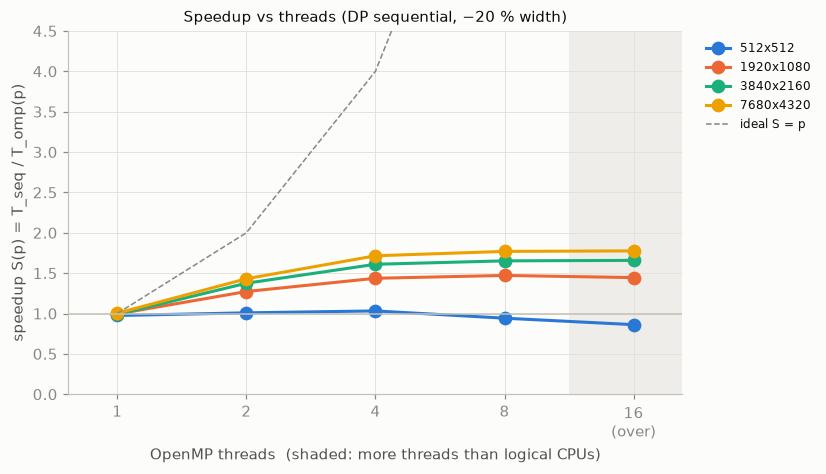
\includegraphics[width=0.72\textwidth]{speedup_vs_threads_main_nodp.png}
  \caption{M2 with the DP kept sequential, Platform A (Windows).}
  \label{fig:m2nodp}
\end{figure}

\begin{table}[ht]
\centering\footnotesize
\begin{tabular}{@{}lrrrr@{}}
\toprule
Image (seams) & seq (s) & all four parallel, 4 thr. & DP seq., 4 thr. & DP seq., 8 thr. \\
\midrule
$512\times512$ (102) & 0.062 / 0.064 & 2.478\,s (0.03\x) & 0.062\,s (1.03\x) & 0.068\,s (0.94\x) \\
$1920\times1080$ (384) & 2.002 / 1.934 & 20.317\,s (0.10\x) & 1.347\,s (1.44\x) & 1.315\,s (1.47\x) \\
$3840\times2160$ (768) & 16.220 / 16.078 & 83.660\,s (0.19\x) & 9.987\,s (1.61\x) & 9.731\,s (1.65\x) \\
$7680\times4320$ (768 / 1536) & 70.942 / 132.445 & 184.084\,s (0.39\x) & 77.220\,s (1.72\x) & 74.854\,s (1.77\x) \\
\bottomrule
\end{tabular}
\caption{M2 on Platform A (median \texttt{t\_total}; the two sequential values belong to the two
experiments, which differ in the reduction for $7680\times4320$).}
\label{tab:m2}
\end{table}

With the DP in parallel the program is slower than the sequential program in every configuration (speedup
0.01--0.68), and \textbf{more threads make it slower}. With the DP kept sequential it reaches
1.40--1.79\x{} for $1920\times1080$ and larger.

\subsection{Why the parallel DP fails on Windows}
\label{sec:why}

\begin{figure}[ht]
  \centering
  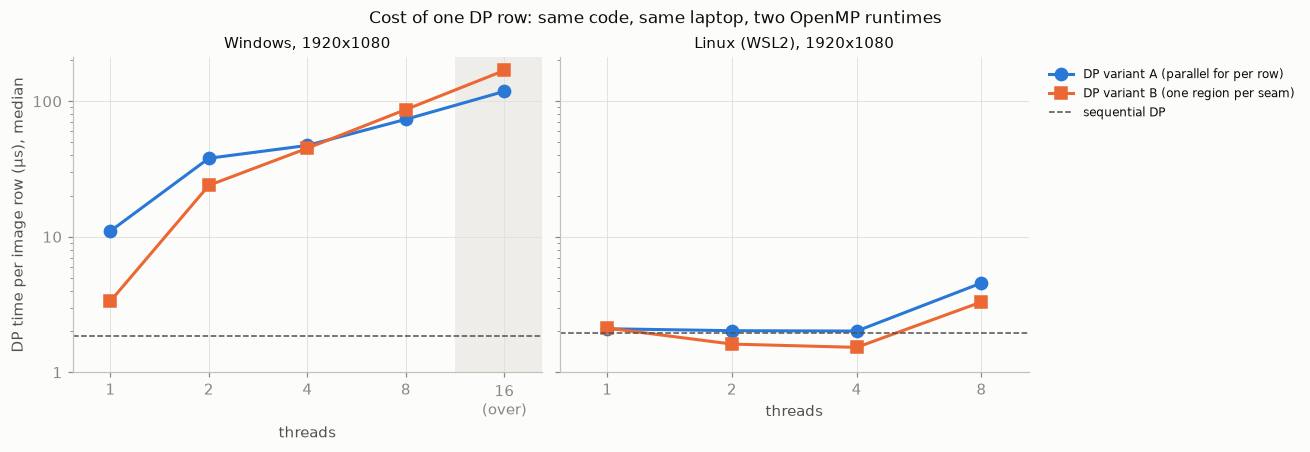
\includegraphics[width=0.72\textwidth]{dp_time_per_row.png}
  \caption{DP time per image row, Platform A.}
\end{figure}

One DP row of an average width of 1728 pixels contains 1.84\us{} of work ($\approx1.06$\,ns per cell). On
Windows, the per-row synchronization adds 9.2\us{} even with one thread (entering and leaving a parallel
region) and 22--167\us{} with 2--16 threads. With 4 threads, \num{414336} synchronizations $\times$
45\us{} $\approx$ 18.8\,s \calc{} explain the measured DP time of 19.6\,s. A simple model,
\[
  t_{\text{row}}(p) \approx \frac{w\,W}{p} + o(p),
\]
shows that the parallel DP pays off only if $w\,W\,(1-1/p) > o(p)$: on Windows ($o(4)\approx45$\us) for
images wider than about \num{56000} pixels, under Linux ($o(4)\approx1.0$--$1.5$\us) for widths above
1\,200--1\,800 pixels \calc. The supplementary Linux run on the same laptop confirmed this: the parallel DP
became as fast as or faster than the sequential DP (up to 1.27\x{} at $1920\times1080$, variant B), and all
four stages in parallel reached 1.36--1.71\x{} with 4 threads. \textbf{The slowness is caused by the
OpenMP runtime on Windows, not by the algorithm.}

\subsection{Optimized version (M5), Platform B}

\begin{table}[ht]
\centering\small
\begin{tabular}{@{}lrrrrrr@{}}
\toprule
Image & seq (s) & M2 best (8 thr.) & M5, 1 thr. & M5, 4 thr. & M5, 8 thr. & M5, 16 thr. \\
\midrule
$512\times512$, $-20\,\%$ & 0.066 & 1.63\x & 2.39\x & 3.21\x & \textbf{3.36\x} & 0.98\x \\
$1920\times1080$, $-20\,\%$ & 2.213 & 1.61\x & 2.37\x & 4.19\x & \textbf{4.64\x} & 3.60\x \\
$3840\times2160$, $-20\,\%$ & 16.388 & 1.48\x & 2.37\x & 4.13\x & \textbf{4.40\x} & 3.85\x \\
$7680\times4320$, $-10\,\%$ & 66.038 & 1.55\x & 2.49\x & 4.43\x & \textbf{4.69\x} & 4.11\x \\
\bottomrule
\end{tabular}
\caption{Speedup over the sequential program on Platform B (``M2 best'' = energy + minimum + removal
parallel, DP sequential). The maximum, 4.76\x, was measured at $1920\times1080$ with 12 threads.}
\label{tab:m5}
\end{table}

\begin{figure}[ht]
  \centering
  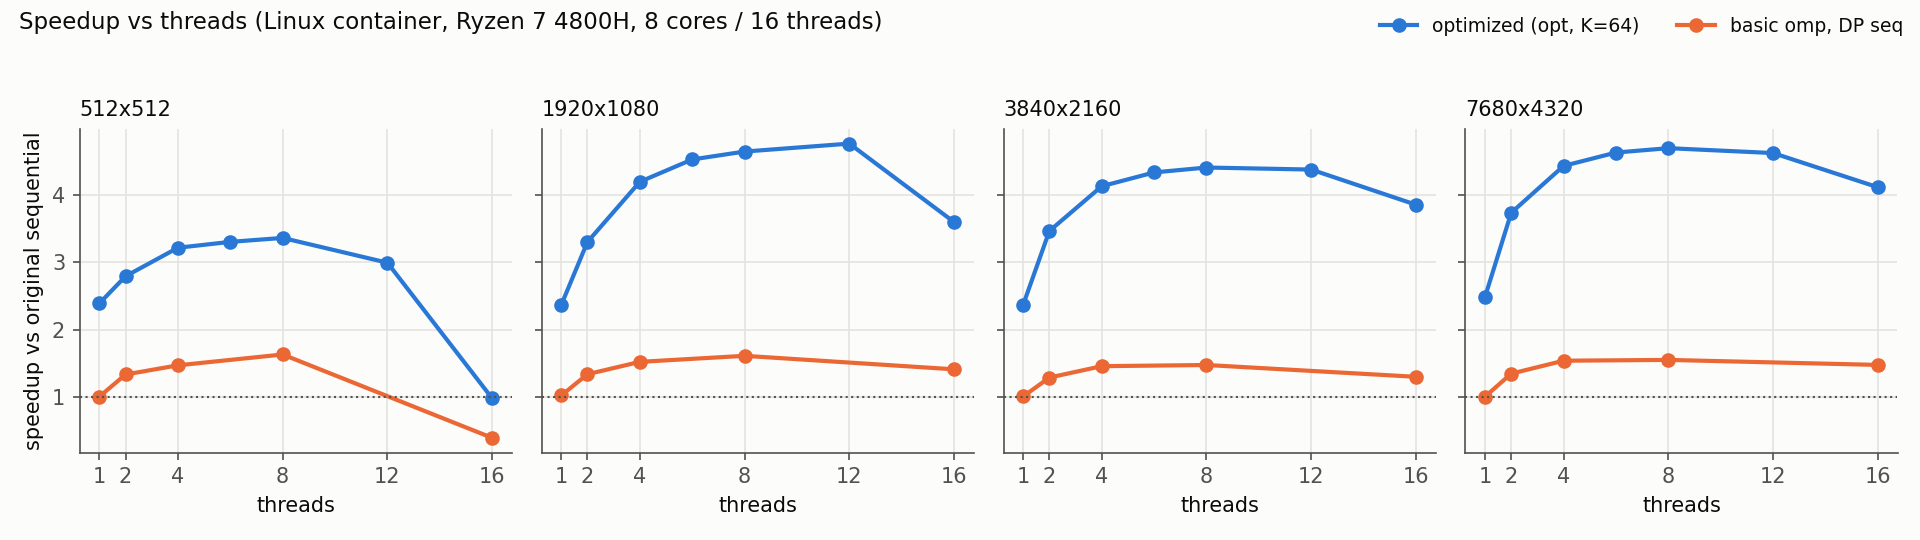
\includegraphics[width=\textwidth]{m5_speedup_threads.png}
  \caption{Speedup over the sequential program, optimized version (blue) and best M2 configuration
  (orange), Platform B.}
\end{figure}

On the five other scenes ($1920\times1080$, 8 threads) the speedup ranges from 4.18\x{} to 6.33\x; all
outputs are identical to the sequential outputs.

% ---------------------------------------------------------------------------
\section{Speedup and Efficiency Analysis}

Speedup $S(p)=T_{\text{seq}}/T(p)$; efficiency $E(p)=S(p)/p$.

\paragraph{Decomposition of the M5 speedup.} The optimized version is 2.37--2.49\x{} faster than the
sequential program \emph{with one thread}, because it does less work (Section~\ref{sec:opt}). From 1 to 8
threads it gains a further 1.9--2.0\x. The total of 4.4--4.8\x{} is the product of both. Measured against
its own one-thread time, the efficiency at 8 threads is therefore only $\approx0.25$; measured against the
sequential program, $E(8)=0.42$--$0.59$. Both views are reported because both are common, and they answer
different questions: the first measures parallel scalability, the second the benefit for the user.

\paragraph{Amdahl's law for M2.} With the DP sequential, the serial fraction on Platform A at
$1920\times1080$ is at least the DP share, $f\approx0.39$--$0.40$. The bound $1/(f+(1-f)/p)$ gives 1.82\x{}
for $p=4$ and 2.11\x{} for $p=8$ \calc; the measured 1.44\x{} and 1.47\x{} are below the bound because the
parallel stages themselves do not scale linearly (energy 3.3--3.6\x, removal $\approx1.1$\x{} at this
size). As $p\to\infty$ the bound is $1/f\approx2.5$\x: \textbf{M2 can never exceed about 2.5\x{} without
parallelizing the DP.} M5 removes this limit by making the DP parallel and cheap.

\paragraph{Saturation.} In M5 most of the gain is reached with 4 threads; 8--12 threads add 5--15\,\%. Two
stages remain after the optimizations, the DP and the removal (Table~\ref{tab:stages8k}), and both are
memory-bound (Section~\ref{sec:membw}).

\begin{table}[ht]
\centering\small
\begin{tabular}{@{}lrrrrr@{}}
\toprule
$7680\times4320$ & 1 thread & 2 & 4 & 8 & 16 \\
\midrule
DP (s) & 16.54 & 10.00 & 7.27 & 5.93 & 7.28 \\
removal (s) & 9.67 & 7.34 & 7.34 & 7.91 & 8.41 \\
total (s) & 26.57 & 17.69 & 14.91 & 14.08 & 16.06 \\
\bottomrule
\end{tabular}
\caption{Stage times of the optimized version at $7680\times4320$.}
\label{tab:stages8k}
\end{table}

\paragraph{Size dependence.} Larger images give more work per synchronization, so the efficiency increases
with the image size (M4: 1.03 $\to$ 1.44 $\to$ 1.61 $\to$ 1.72 with 4 threads, DP sequential). For
$512\times512$ the M5 version still gains 3.36\x{} with 8 threads under Linux, but collapses with 16
threads (0.98\x, highly variable).

% ---------------------------------------------------------------------------
\section{Bottlenecks and Limitations}
\label{sec:bottle}

\subsection{Synchronization}
Per-row barriers make a fine-grained wavefront DP impractical on platforms with expensive synchronization
(Section~\ref{sec:why}). Even under Linux, where a barrier costs about 1\us, a $512\times512$ image has only
about 0.5\us{} of DP work per row (\emph{calculation}: 512 cells $\times\approx1$\,ns).

\subsection{Memory bandwidth}
\label{sec:membw}
Every stage performs only a few operations per byte. Platform B sustains 34--35\,GB/s for reading,
12.7\,GB/s for writing and 19.1--19.6\,GB/s for copying with 8 threads (\texttt{results/m5\_membw.txt}).
Two observations follow:
\begin{itemize}
  \item \emph{DP.} With a full 32-bit $M$ matrix, the DP touches $\approx12$ bytes per cell and its working
    set at $1920\times1080$ ($\approx16.6$\,MB) exceeds the 8\,MB L3 cache \calc; the blocked parallel DP
    then gains almost nothing (0.547 $\to$ 0.512\,s). After the compact-memory optimization the working
    set is $\approx6.2$\,MB and the same parallel DP halves the time (0.580 $\to$ 0.287\,s).
  \item \emph{Removal.} At $7680\times4320$ with 8 threads, the seam removal moves an estimated 145\,GB in
    7.91\,s $\approx$ 18\,GB/s (\emph{calculation}, seams assumed uniformly distributed), i.e.\ close to the
    measured copy bandwidth. More threads cannot speed it up, and it is now the largest stage.
\end{itemize}

\subsection{Simultaneous multithreading}
16 threads on 8 cores are slower than 8 threads in every configuration on Platform B, and highly variable
on small images (0.043--0.337\,s for $512\times512$). Two hardware threads of a core share its caches and
load/store units, and every barrier waits for the slowest thread.

\subsection{Inherently sequential parts}
The seam loop, the backtracking and the minimum remain sequential. Their share is small ($<3\,\%$), but it
grows as the parallel stages get faster.

\subsection{Limitations of the study}
\begin{itemize}
  \item Two different machines and operating systems for M4 and M5; M5 was measured in a container on a
    virtualized Linux kernel (WSL2), not natively on Windows.
  \item One compiler family (GCC/libgomp) for all performance results; clang/libomp was used only for the
    ThreadSanitizer checks.
  \item Memory-traffic arguments are calculations; hardware performance counters were not available in the
    container.
  \item Only the basic $e_1$ energy and seam removal are implemented (no forward energy, no enlarging, no
    optimal seam order).
\end{itemize}

% ---------------------------------------------------------------------------
\section{Optimization}
\label{sec:opt}

Every optimization of the M5 version (\texttt{src/seam\_opt.cpp}, \texttt{--mode opt}) can be switched off
and was measured against the previous step (\texttt{docs/optimization\_report.md}).
Figure~\ref{fig:ablation} and Table~\ref{tab:chain} show the step chain.

\begin{figure}[ht]
  \centering
  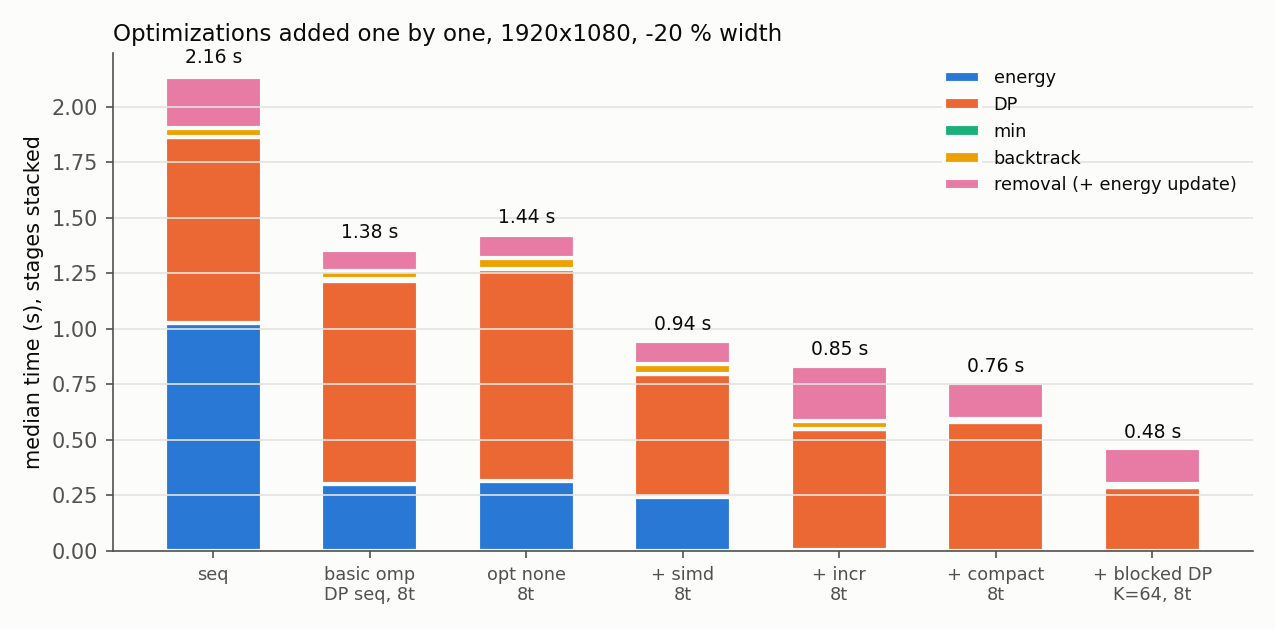
\includegraphics[width=0.8\textwidth]{m5_ablation_1920x1080.png}
  \caption{Stage times when the optimizations are added one by one, $1920\times1080$, 8 threads,
  Platform B.}
  \label{fig:ablation}
\end{figure}

\begin{table}[ht]
\centering\small
\begin{tabular}{@{}lrr@{}}
\toprule
Step (8 threads, $1920\times1080$) & total (s) & speedup vs.\ seq \\
\midrule
sequential & 2.160 & 1.00 \\
M2, DP sequential & 1.378 & 1.57 \\
M5, all optimizations off & 1.435 & 1.51 \\
+ SIMD kernels (O2) & 0.944 & 2.29 \\
+ incremental energy (O1) & 0.850 & 2.54 \\
+ compact memory (O5) & 0.764 & 2.83 \\
+ blocked DP, $K=64$ (O3) & \textbf{0.479} & \textbf{4.51} \\
\bottomrule
\end{tabular}
\caption{Step chain (median of 5 runs).}
\label{tab:chain}
\end{table}

\subsection{O2 -- Vectorizable kernels}
Only the border columns need index clamping. Treating columns 0 and $W-1$ separately leaves a branch-free
interior loop that the compiler vectorizes under \texttt{\#pragma omp simd}. One thread: energy 2.8\x, DP
1.7\x{} faster.

\subsection{O1 -- Incremental energy}
\textbf{Claim.} After removing seam pixel $s=s(y)$ from row $y$, only the new columns $s-1$ and $s$ of row
$y$ can change their energy. \emph{Argument.} The energy at new column $x$ depends on columns $x\pm1$ of row
$y$ and column $x$ of rows $y\pm1$, whose seam positions differ from $s$ by at most one. For $x\le s-2$ all
four pixels lie left of every involved seam and are unchanged; for $x\ge s+1$ all four pixels moved one
position left, so the energy equals the old energy at $x+1$, which the shift moves along. The energy is
therefore computed once, shifted with the image, and two values per row are recomputed:
\begin{lstlisting}[style=cpp]
#pragma omp parallel if(par)
{
    #pragma omp for schedule(runtime)
    for (int y = 0; y < height; ++y) removeRow(image, gray, energy, width, seam[y], y);
    // implicit barrier: all rows are shifted before rows y-1 and y+1 are read below
    #pragma omp for schedule(runtime)
    for (int y = 0; y < height; ++y)
        energyRowRange(gray, width - 1, *energy, y, max(0, s-1), min(width-1, s+1), false);
}
\end{lstlisting}
The claim is verified after every seam against a full recomputation (\texttt{tests/test\_opt.cpp}). The
energy stage drops from 1.110\,s to 0.007\,s (one thread), while the removal doubles because it shifts the
energy map too.

\subsection{O3 -- Blocked DP with halo computation}
\label{sec:o3}
Rows are processed in blocks of $K$. Thread $t$ owns columns $[a,b)$. In local row $j=0,\dots,K-1$ of a
block it computes, in private buffers, the widened range
\[
  \bigl[a-(K-1-j),\; b+(K-1-j)\bigr),
\]
which shrinks by one column per side per row and equals its own range in the last row
(Figure~\ref{fig:halo}). The first row of the block reads the complete last row of the previous block,
which is guaranteed by \textbf{one barrier per block}. Every cell is computed with the same inputs as in the
sequential DP, so $M$ is identical.

\begin{figure}[ht]
\centering
\begin{tikzpicture}[x=0.36cm,y=0.42cm]
  % K = 4 rows, own columns [8,14)
  \def\a{8}\def\b{14}\def\K{4}
  \foreach \j in {0,...,3} {
    \pgfmathtruncatemacro{\h}{\K-1-\j}
    \pgfmathtruncatemacro{\lo}{\a-\h}
    \pgfmathtruncatemacro{\hi}{\b+\h}
    \fill[warn!25] (\lo,-\j) rectangle (\a,-\j-1);
    \fill[warn!25] (\b,-\j) rectangle (\hi,-\j-1);
    \fill[accent!35] (\a,-\j) rectangle (\b,-\j-1);
    \node[font=\scriptsize, anchor=east] at (2.6,-\j-0.5) {$j=\j$};
  }
  \draw[gray!60, step=1] (3,0) grid (19,-4);
  \fill[gray!25] (3,1.2) rectangle (19,0.2);
  \draw[gray!60] (3,1.2) grid (19,0.2);
  \node[font=\scriptsize, anchor=west] at (19.3,0.7) {last row of previous block (shared)};
  \draw[very thick, warn] (3,-4.35) -- (19,-4.35);
  \node[font=\scriptsize, anchor=west, text=warn] at (19.3,-4.35) {\textbf{barrier} (one per block)};
  \draw[|-|, accent] (\a,-4.9) -- (\b,-4.9);
  \node[font=\scriptsize] at (11,-5.5) {own columns $[a,b)$ of one thread};
  \node[font=\scriptsize, anchor=west] at (19.3,-1.2) {\textcolor{accent!70}{\rule{6pt}{6pt}} own cells (published)};
  \node[font=\scriptsize, anchor=west] at (19.3,-2.4) {\textcolor{warn!60}{\rule{6pt}{6pt}} halo cells (private)};
\end{tikzpicture}
\caption{Blocked DP for $K=4$: the halo shrinks by one column per side per row, so the last row of the block
depends only on cells the thread computed itself.}
\label{fig:halo}
\end{figure}

\begin{lstlisting}
parallel region:
    [a, b) <- my columns
    for each block of rows y0 .. y0+K-1:
        prev <- shared last row of previous block, columns [a-K, b+K)
        for j in 0 .. K-1:
            lo <- a-(K-1-j);  hi <- b+(K-1-j)          // clipped to [0, W)
            cur[lo:hi] <- e[y0+j][lo:hi] + min3(prev)  // private buffer
            publish cur[a:b] (directions, last row)    // own columns only
            swap(prev, cur)
        barrier                                         // one per block
\end{lstlisting}

Barriers per seam fall from $H$ to $H/K$; the redundant work is about $K-1$ cells per row and thread
($\approx1\,\%$ for $K=64$, 1920 columns, 8 threads; \emph{calculation}). The DP time drops monotonically up
to $K\approx16$ and is flat between 16 and 256 (Figure~\ref{fig:block}); $K=64$ is the default.

\begin{figure}[ht]
  \centering
  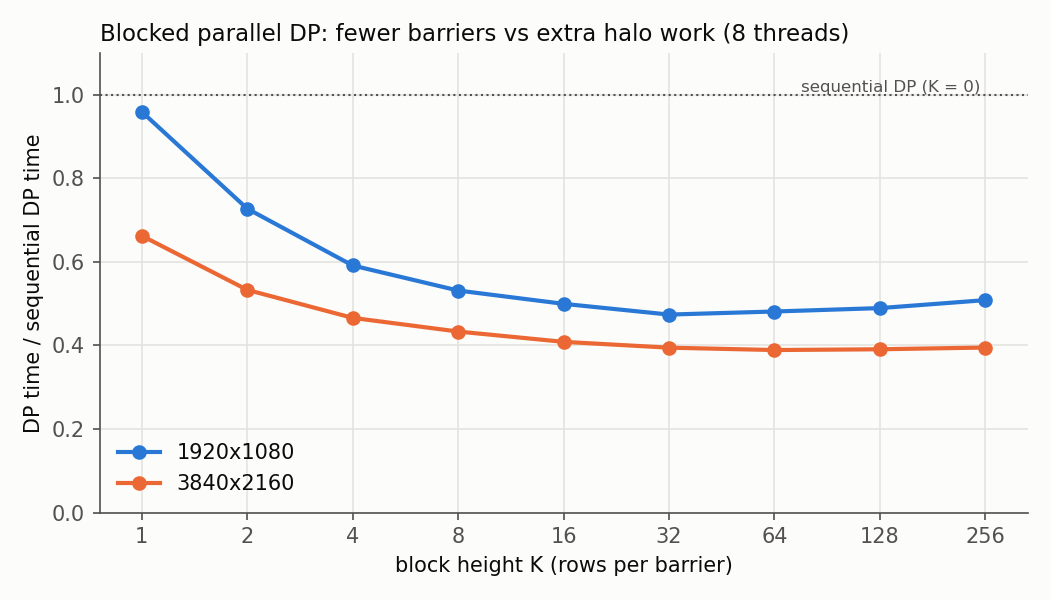
\includegraphics[width=0.72\textwidth]{m5_dp_block.png}
  \caption{DP time relative to the sequential DP versus block height $K$, 8 threads, Platform B.}
  \label{fig:block}
\end{figure}

\subsection{O5 -- Compact memory}
The energy fits into 16 bits (maximum 510). Backtracking needs only the direction ($-1$, 0, $+1$) of the
best upper neighbour, which is stored in one byte per pixel; $M$ is kept in two rolling rows, and the last
row is saved for the minimum search. The direction uses the sequential tie rule, so the seam is unchanged:
\texttt{seam[y-1] = seam[y] + dir[y][seam[y]]}. This reduces the DP working set from $\approx16.6$\,MB to
$\approx6.2$\,MB at $1920\times1080$ and is what makes O3 effective (Section~\ref{sec:membw}): with 8
threads, total time 0.845 $\to$ 0.479\,s when O5 is added to O1 + O2 + O3.

\subsection{Optimizations not adopted}
\begin{itemize}
  \item \textbf{Size threshold} (\texttt{if} clause below $N$ pixels): no gain at $\le12$ threads on Linux,
    because even $512\times512$ benefits from 8 threads; kept as an option, default off.
  \item \textbf{Schedules} \texttt{static,1}, \texttt{dynamic,16}, \texttt{guided}: within the run-to-run
    noise ($\le5\,\%$); every row has the same cost, so there is no load imbalance to correct.
    \texttt{static} is kept.
  \item \textbf{Parallel minimum and backtracking}: M4 measured the parallel minimum 8--100\x{} slower;
    backtracking is a dependent chain.
\end{itemize}

\subsection{Verification of the optimized version}
\label{sec:verify}
\texttt{tests/test\_opt.cpp} compares every kernel (energy 32/16-bit, DP, directions for
$K\in\{0,1,2,3,4,5,8,16,31,64,1000\}$, incremental update) and the whole \texttt{carve} with the
sequential code for 1--16 threads: \num{18636} checks, 0 failed, also under AddressSanitizer/UBSan. Ten
mutants (e.g.\ removed block barrier, halo one cell short, removed removal barrier, wrong tie rule, single
shared boundary row) are all detected. ThreadSanitizer with the Archer OpenMP tool (clang 18, LLVM libomp)
reports \textbf{no data race} on the original code (\texttt{test\_opt} full, \num{18636} checks), and 290
data-race reports in \texttt{src/seam\_opt.cpp} when the block barrier is removed (positive control, 612
failed checks).

% ---------------------------------------------------------------------------
\section{Conclusion and Future Work}

Seam carving offers parallelism only inside each seam, and its most expensive stage, the DP, needs a
synchronization per image row. A direct OpenMP parallelization therefore depends heavily on the cost of a
barrier: on Windows with GCC's libgomp it made the program up to 100\x{} slower, while under Linux it gave
a modest gain. Keeping the DP sequential limits the speedup to about 2.5\x{} by Amdahl's law; measured,
1.4--1.8\x.

The optimized version shows that the decisive factors are \textbf{work avoidance} and \textbf{memory
traffic}, not the number of threads: one thread of the optimized code is already 2.4\x{} faster than the
original, the blocked DP is useful only once the data of the DP fits into the cache, and the remaining
bottleneck, the seam removal, runs at close to the memory copy bandwidth. The final result is
4.4--4.8\x{} over the sequential program with 8 threads on an 8-core laptop, with outputs that are
bit-identical to the sequential program in every one of \num{1905} benchmark runs and about \num{237000}
test checks ($65+\num{147368}+\num{71580}+\num{18636}$ in the four full test programs).

Future work:
\begin{enumerate}
  \item Avoid the physical pixel shift, e.g.\ by removing several non-overlapping seams per pass or by an
    index-based representation; this would change the algorithm and needs new correctness arguments.
  \item Forward energy~\cite{rubinstein2008} and seam insertion.
  \item Native Windows measurements with a different OpenMP runtime (e.g.\ LLVM libomp) to separate runtime
    effects from hardware effects.
  \item Hardware-counter measurements (cache misses, bandwidth) to confirm the memory-traffic calculations.
  \item GPU implementation of the blocked DP, where the halo technique is commonly used.
\end{enumerate}

% ---------------------------------------------------------------------------
\section*{Author Contributions}
\addcontentsline{toc}{section}{Author Contributions}

The project was divided along the seven project milestones (M0--M6) so that no single member
owned the whole parallel implementation or the whole write-up.

\begin{description}[leftmargin=2.2cm, style=nextline, itemsep=4pt]
  \item[Đỗ Tùng Dương] \textbf{M1 -- Sequential implementation} and \textbf{M3 -- Correctness
    validation}: the baseline energy map, dynamic-programming seam search and seam removal
    (\texttt{src/seam\_seq.cpp}), and the full test suite including the sequential-versus-parallel
    equivalence checks (\texttt{tests/}).
  \item[Hoàng Trọng Đại] \textbf{M2 -- OpenMP parallelization} and \textbf{M5 -- Performance
    optimization}: the parallel energy map, DP and seam removal (\texttt{src/seam\_omp.cpp}), and the
    optimized version with incremental energy, blocked DP and compact memory layout
    (\texttt{src/seam\_opt.cpp}).
  \item[Lê Quang Huy] \textbf{M0 -- Project setup}, \textbf{M4 -- Performance benchmarking} and
    \textbf{M6 -- Report and presentation}: the build system and project plan, the reproducible
    benchmark harness and result analysis (\texttt{scripts/}, \texttt{results/}), and this report and
    the slides. Repository maintainer.
\end{description}

All members reviewed the final report and the benchmark results together.

% ---------------------------------------------------------------------------
\begin{thebibliography}{9}
\bibitem{avidan2007} S.~Avidan and A.~Shamir. \emph{Seam Carving for Content-Aware Image Resizing.} ACM
  Transactions on Graphics 26(3), Article 10 (Proceedings of SIGGRAPH 2007), 2007.
\bibitem{rubinstein2008} M.~Rubinstein, A.~Shamir and S.~Avidan. \emph{Improved Seam Carving for Video
  Retargeting.} ACM Transactions on Graphics 27(3), Article 16 (Proceedings of SIGGRAPH 2008), 2008.
\bibitem{openmp52} OpenMP Architecture Review Board. \emph{OpenMP Application Programming Interface,
  Version 5.2.} November 2021.
\bibitem{chapman2008} B.~Chapman, G.~Jost and R.~van der Pas. \emph{Using OpenMP: Portable Shared Memory
  Parallel Programming.} MIT Press, 2008.
\bibitem{amdahl1967} G.~M.~Amdahl. \emph{Validity of the Single Processor Approach to Achieving Large Scale
  Computing Capabilities.} AFIPS Spring Joint Computer Conference, pp.~483--485, 1967.
\bibitem{mccalpin1995} J.~D.~McCalpin. \emph{Memory Bandwidth and Machine Balance in Current High
  Performance Computers.} IEEE Computer Society TCCA Newsletter, December 1995.
\bibitem{williams2009} S.~Williams, A.~Waterman and D.~Patterson. \emph{Roofline: An Insightful Visual
  Performance Model for Multicore Architectures.} Communications of the ACM 52(4), pp.~65--76, 2009.
\bibitem{meng2009} J.~Meng and K.~Skadron. \emph{Performance Modeling and Automatic Ghost Zone Optimization
  for Iterative Stencil Loops on GPUs.} Proceedings of the 23rd International Conference on
  Supercomputing (ICS), 2009.
\end{thebibliography}

\paragraph{Project documents} (detailed evidence for every claim above): \texttt{docs/algorithm.md},
\texttt{docs/parallelization\_strategy.md}, \texttt{docs/architecture.md}, \texttt{docs/testing\_report.md}
(M3), \texttt{docs/benchmark\_report.md} (M4), \texttt{docs/optimization\_report.md} (M5),
\texttt{WORKLOG.md}.

\end{document}
